\documentclass[9pt,ignorenonframetext,mathserif,aspectratio=169,xcolor=dvipsnames]{beamer}
\usetheme{CambridgeUS}
\usepackage[export]{adjustbox}
\usepackage[font={footnotesize}]{caption}
\captionsetup{justification=centering,singlelinecheck=false, labelformat=empty}
\usepackage{amsmath,amsfonts}
\usepackage{graphicx}

\begin{document}

\begin{frame}[t]
	\frametitle{Building a PSHA model}

\begin{columns}[t]

	\column{.55\textwidth}
	\vspace{-0.5cm}
	\only<1-8>{
\begin{itemize}
	\item Combines an Earthquake Occurrence Forecast and a Ground Motion Model
 \end{itemize}
	}
	\only<2-8>{
	\begin{exampleblock}{\large Earthquake Forecasting (Probabilistic)}
\begin{itemize}
	\item Identify potential seismogenic sources
	\item Spatio-temporal distributions of seismicity.
	\item Magnitude-Frequency distributions.
\end{itemize}
\only<5>{
\begin{equation}
    P(N = k) = \frac{\lambda^k e^{-\lambda}}{k!}, \qquad k = 0, 1, 2, \dots
\end{equation}
}
\only<6>{
\begin{equation}
P(N = k) = \frac{\Gamma(k + 1/\alpha)}{\Gamma(1/\alpha)\,k!}\left(\frac{1}{1 + \alpha\lambda}\right)^{\!1/\alpha}\left(\frac{\alpha\lambda}{1 + \alpha\lambda}\right)^{\!k}
\end{equation}
}
	\end{exampleblock}
	\centering
	}
	\only<9-10>{
\begin{alertblock}{\large Ground Motion Model (GMM)}
	\begin{itemize}
\item Ground Shaking Intensity at a site as function of earthquake characteristics and soil conditions
\end{itemize}
	\end{alertblock}
	}
	\only<11>{
		\begin{figure}
		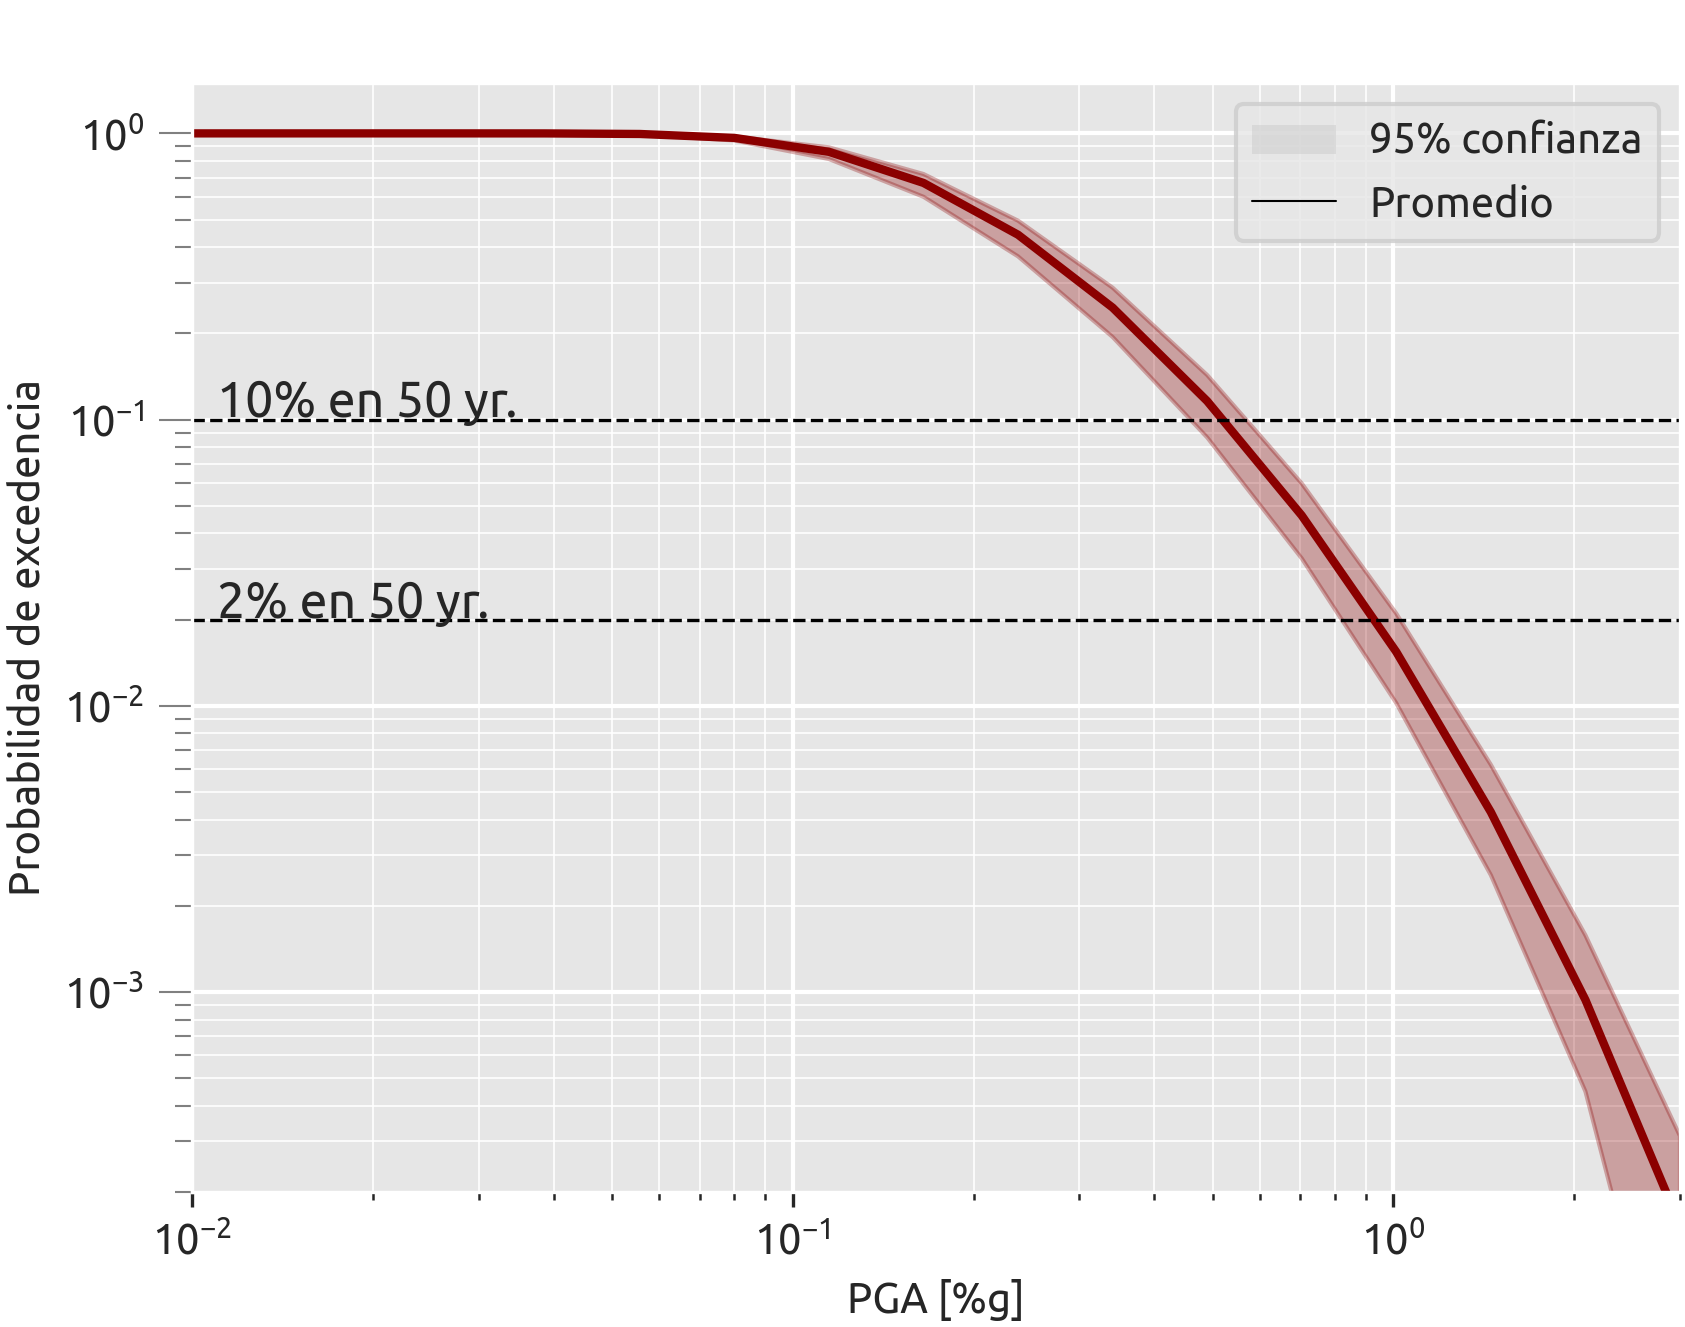
\includegraphics[width=0.85\textwidth]{./figures/curva_2}
		\caption*{\scriptsize Hazard Curve}
	\end{figure}
	}

	\column{.45\textwidth}

	\only<2>{
		\begin{figure}
		\vspace*{-0.5cm}
		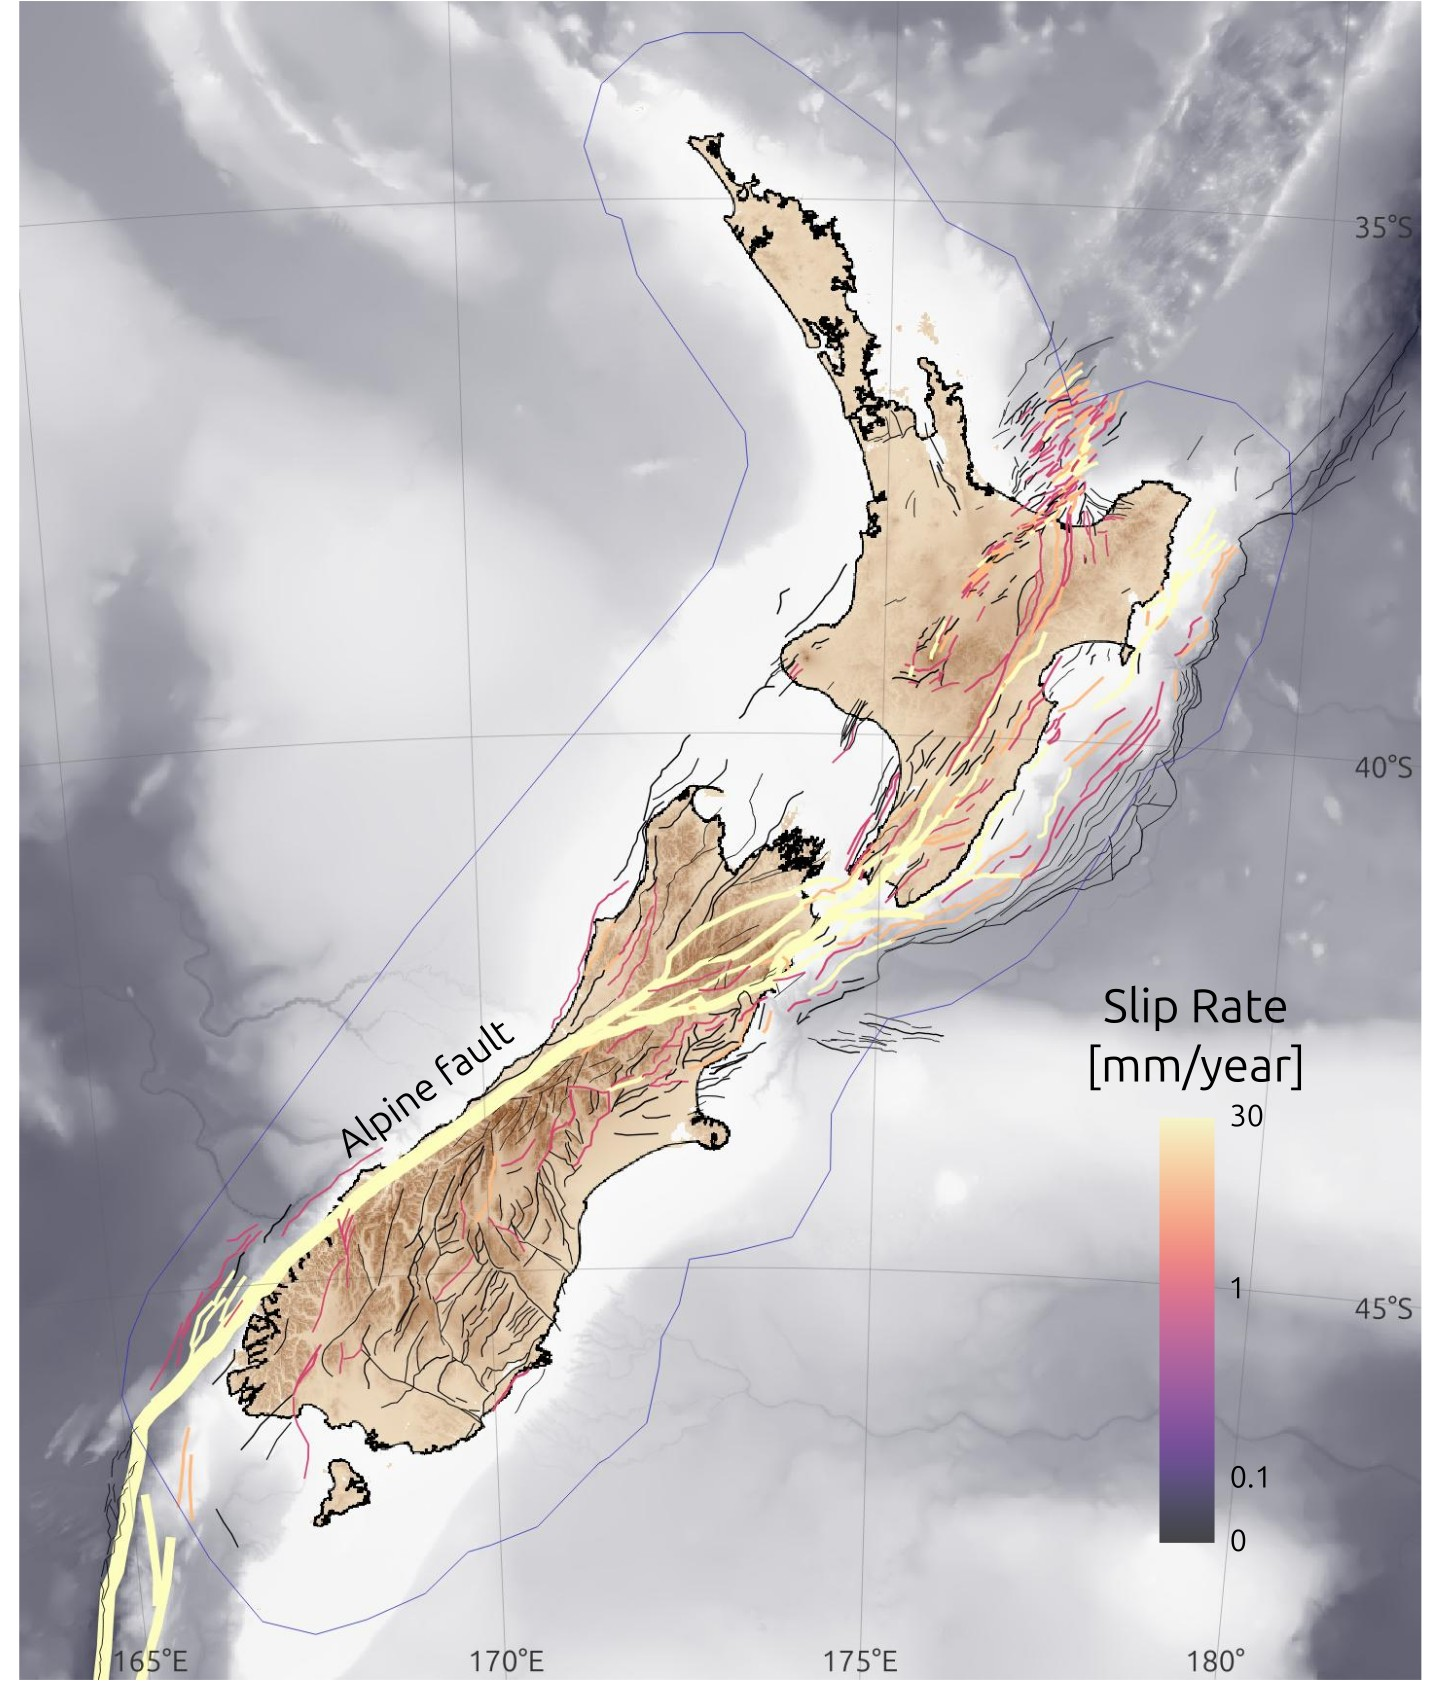
\includegraphics[width=0.85\textwidth]{./figures/faults_map}
		\caption*{\scriptsize Community Fault Model -- New Zealand crustal faults (Seebeck et al., 2025)}
	\end{figure}
	}
	\only<3>{
		\begin{figure}
		\vspace*{-0.5cm}
		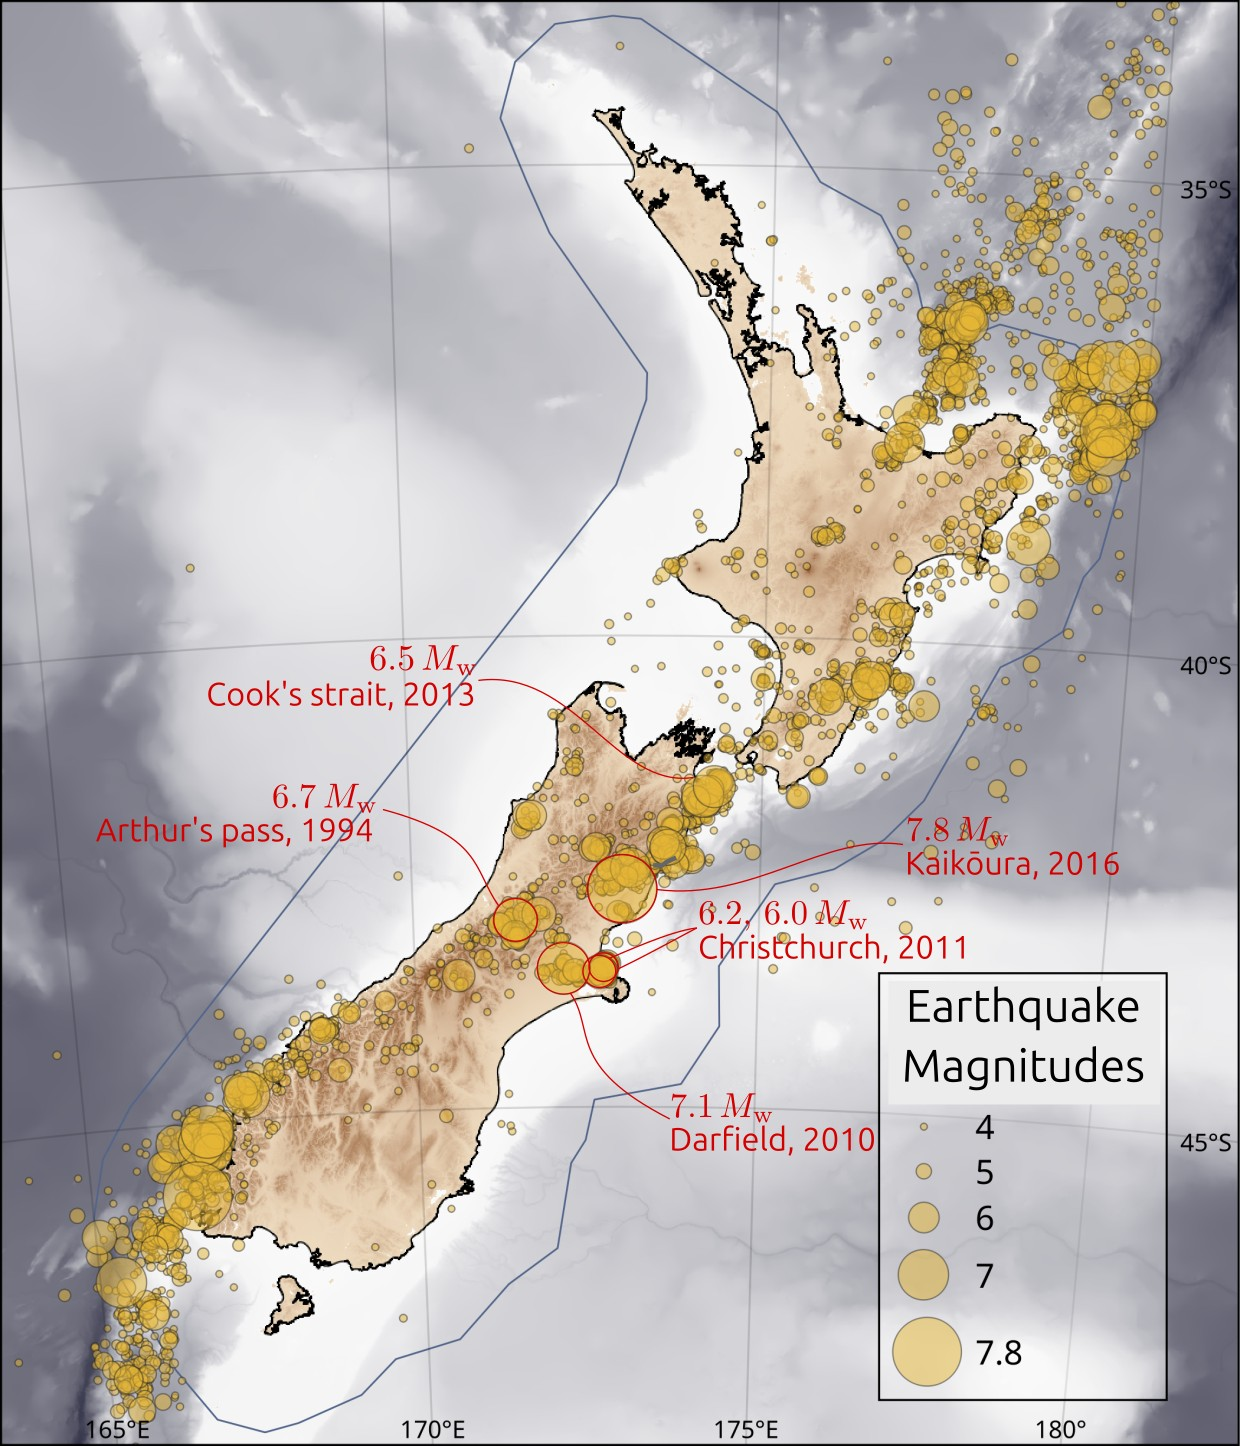
\includegraphics[width=0.85\textwidth]{./figures/catalog_nz}
		\caption*{\scriptsize Seismicity since 1964 (Christophersen et al., 2022)}
	\end{figure}
	}
	\only<4>{
		\begin{figure}
		\vspace*{-1.9cm}
		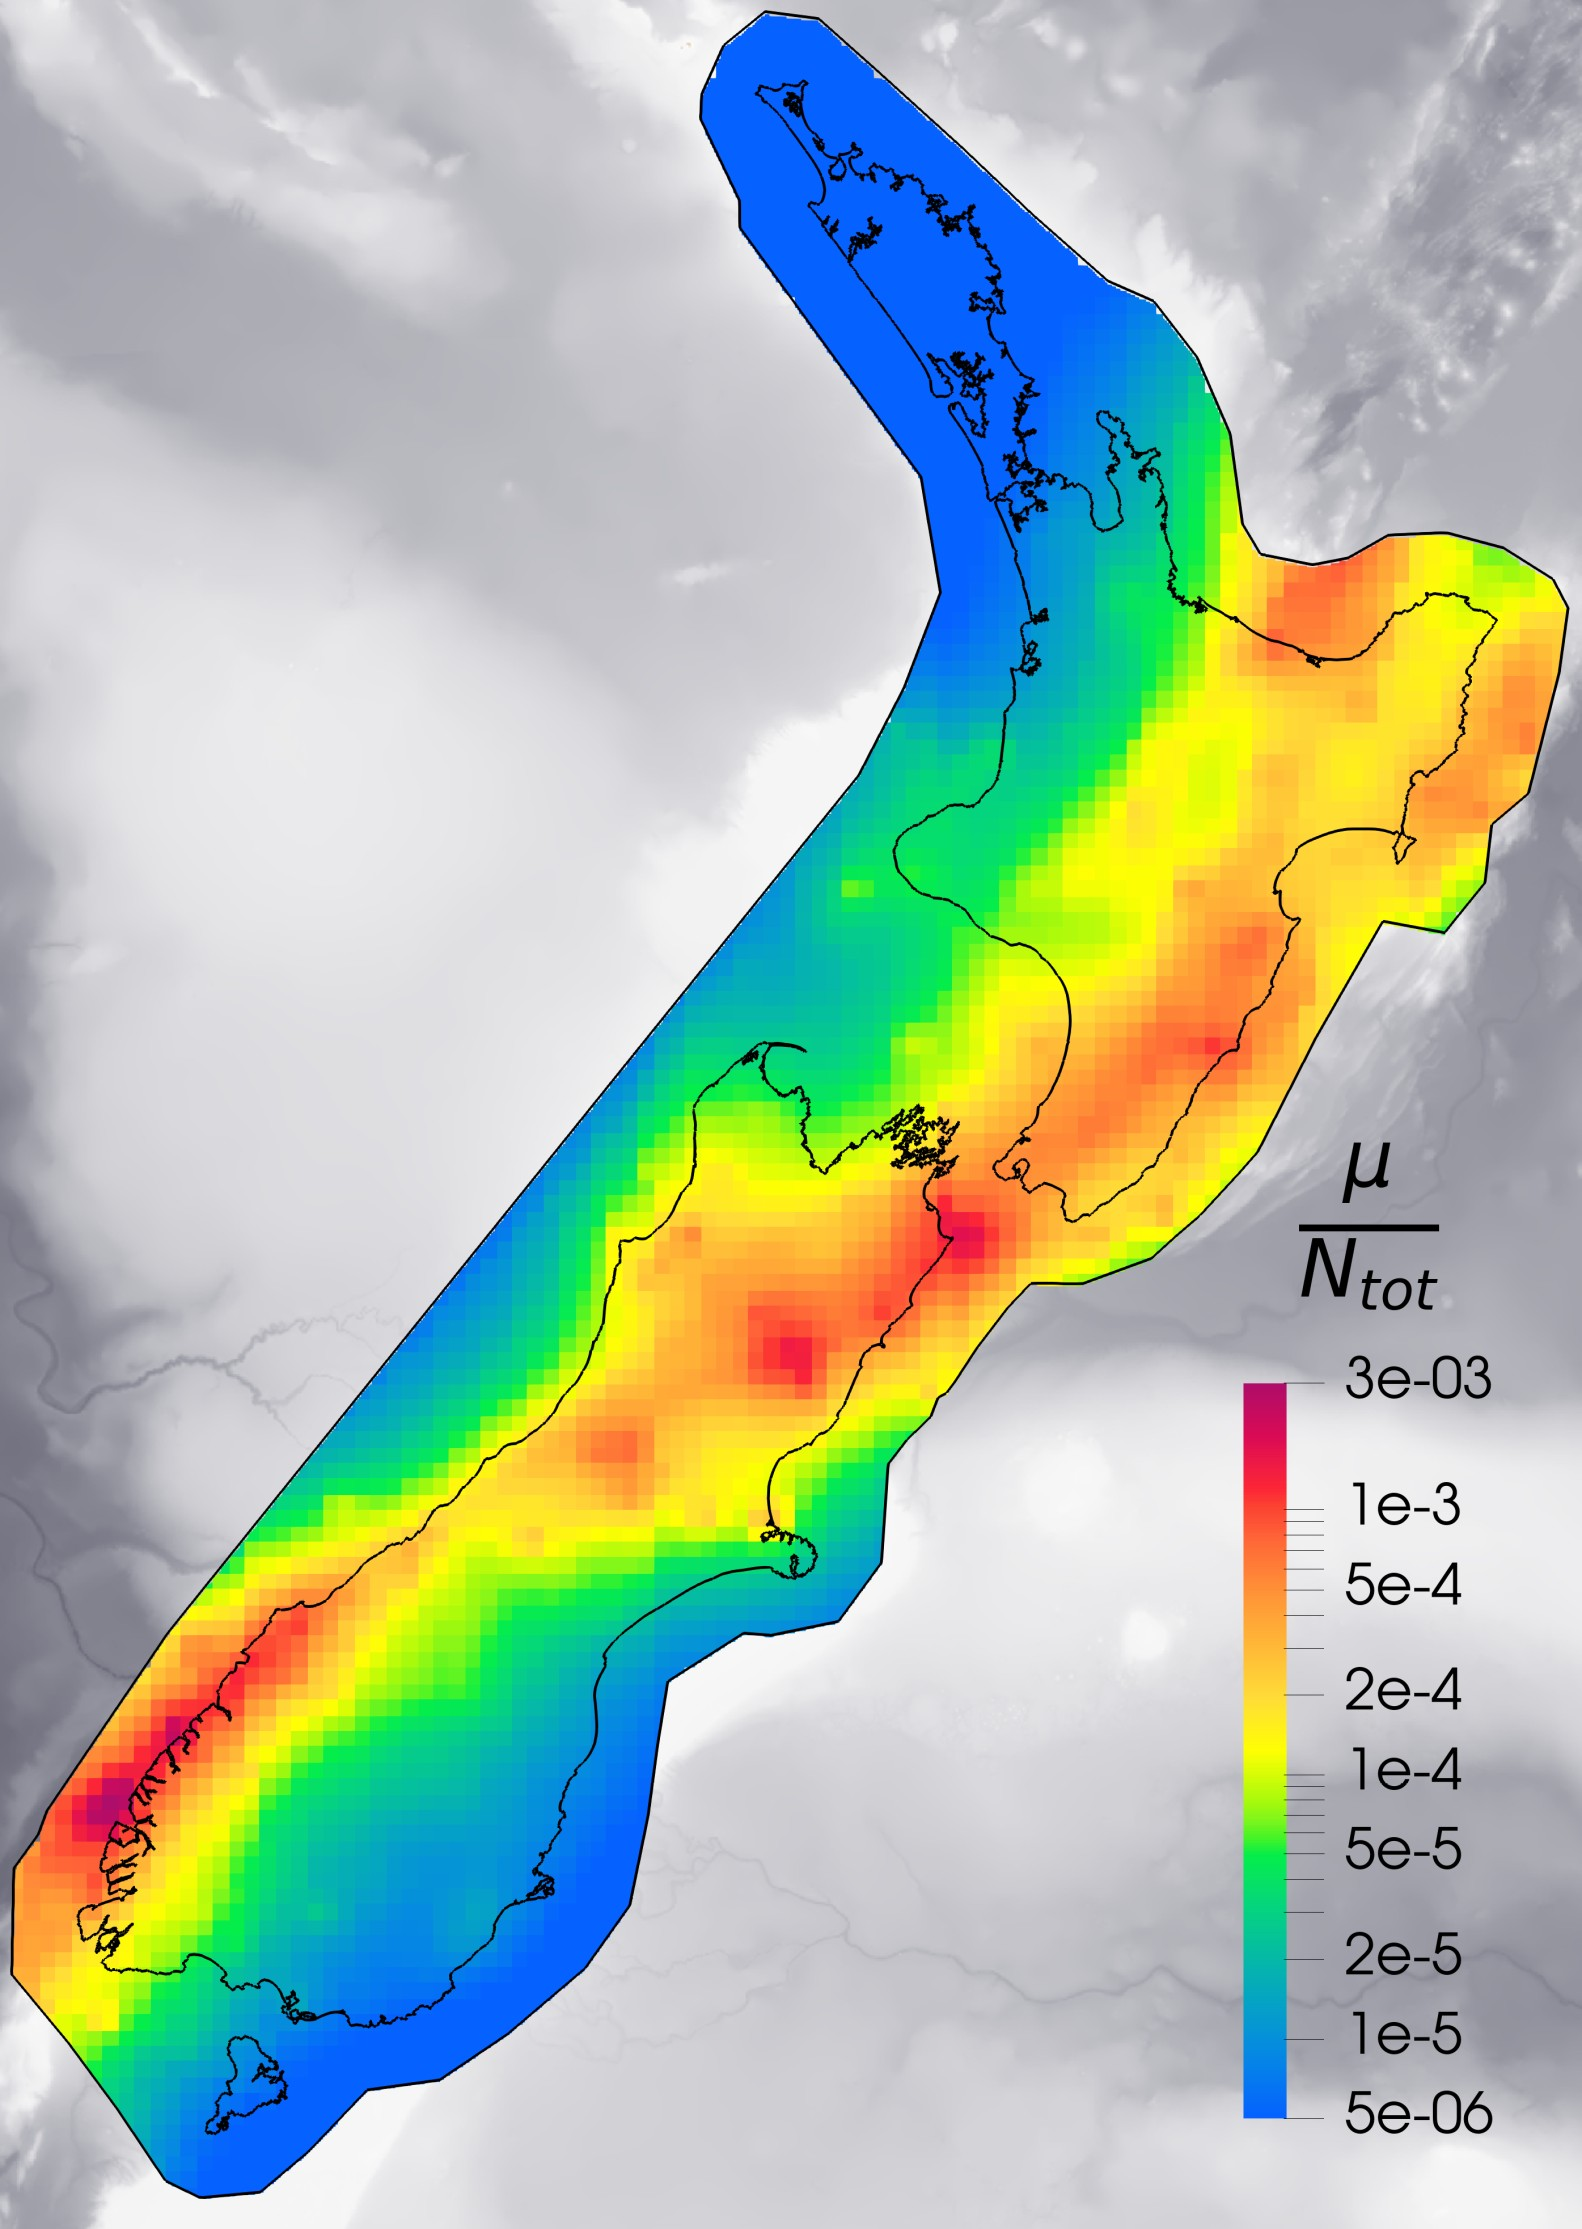
\includegraphics[width=0.8\textwidth]{./figures/gridded1}
		\caption*{Gridded Forecast}
	\end{figure}
	}
	\only<5>{
		\begin{figure}
		\vspace*{-1.9cm}
		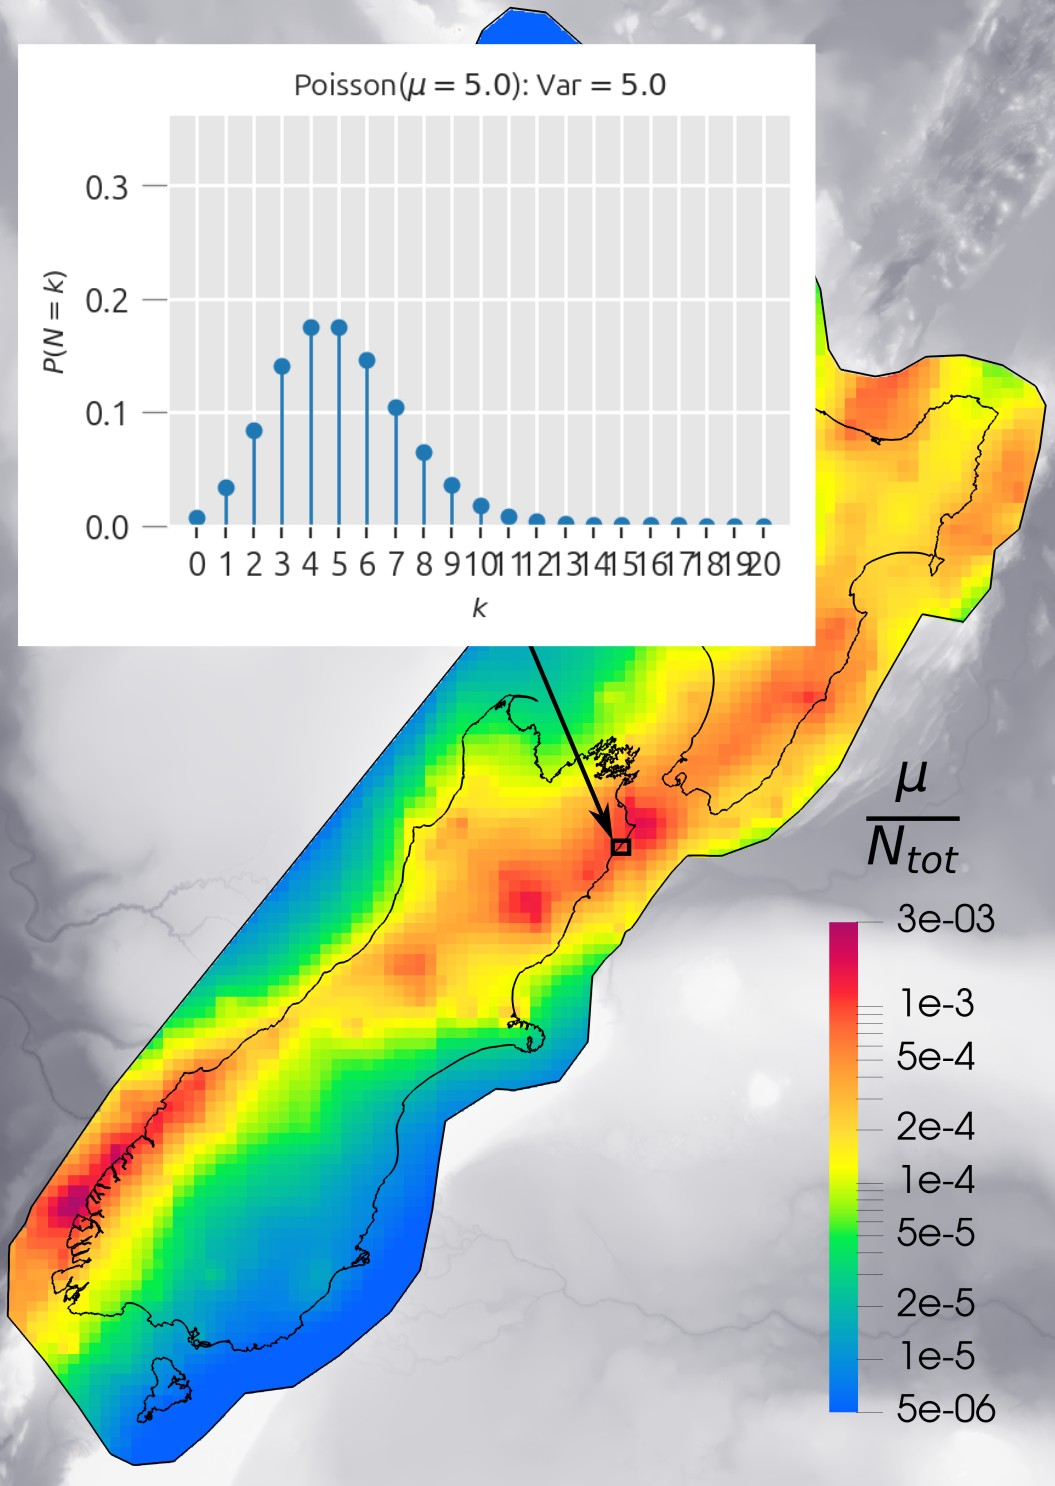
\includegraphics[width=0.8\textwidth]{./figures/gridded2}
		\caption*{Poisson Gridded Forecast}
	\end{figure}
	}
	\only<6>{
		\begin{figure}
		\vspace*{-1.9cm}
		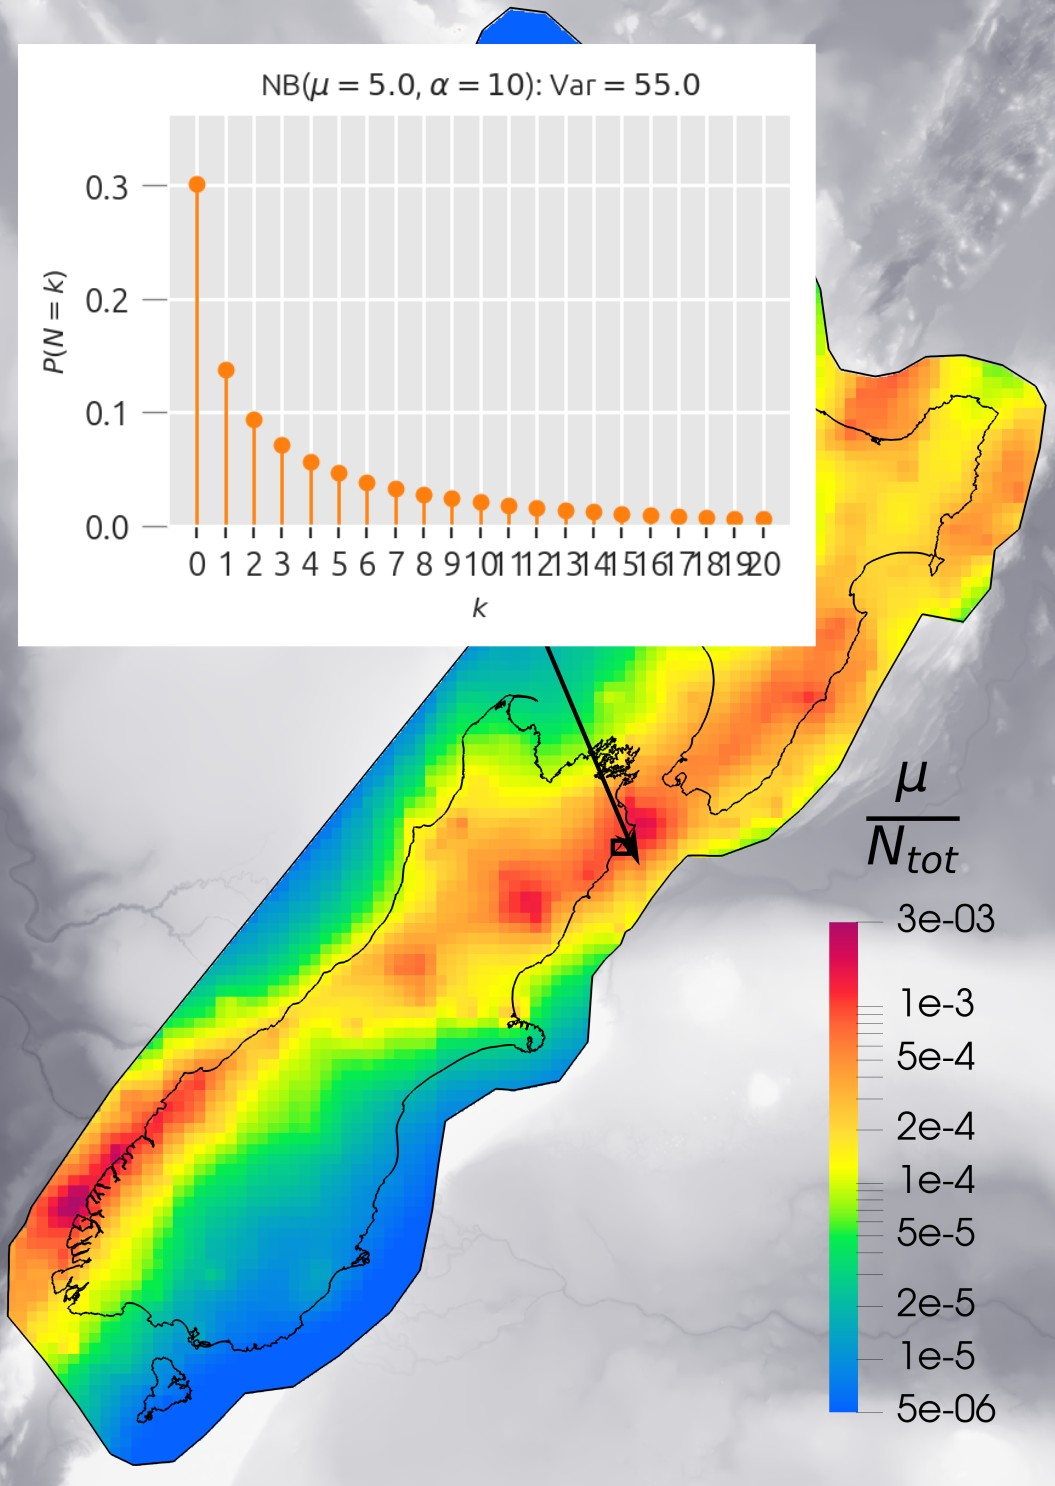
\includegraphics[width=0.8\textwidth]{./figures/gridded3}
		\caption*{Negative Binomial Gridded Forecast}
	\end{figure}
	}
	\only<7>{
		\begin{figure}
		\vspace*{-1.5cm}
		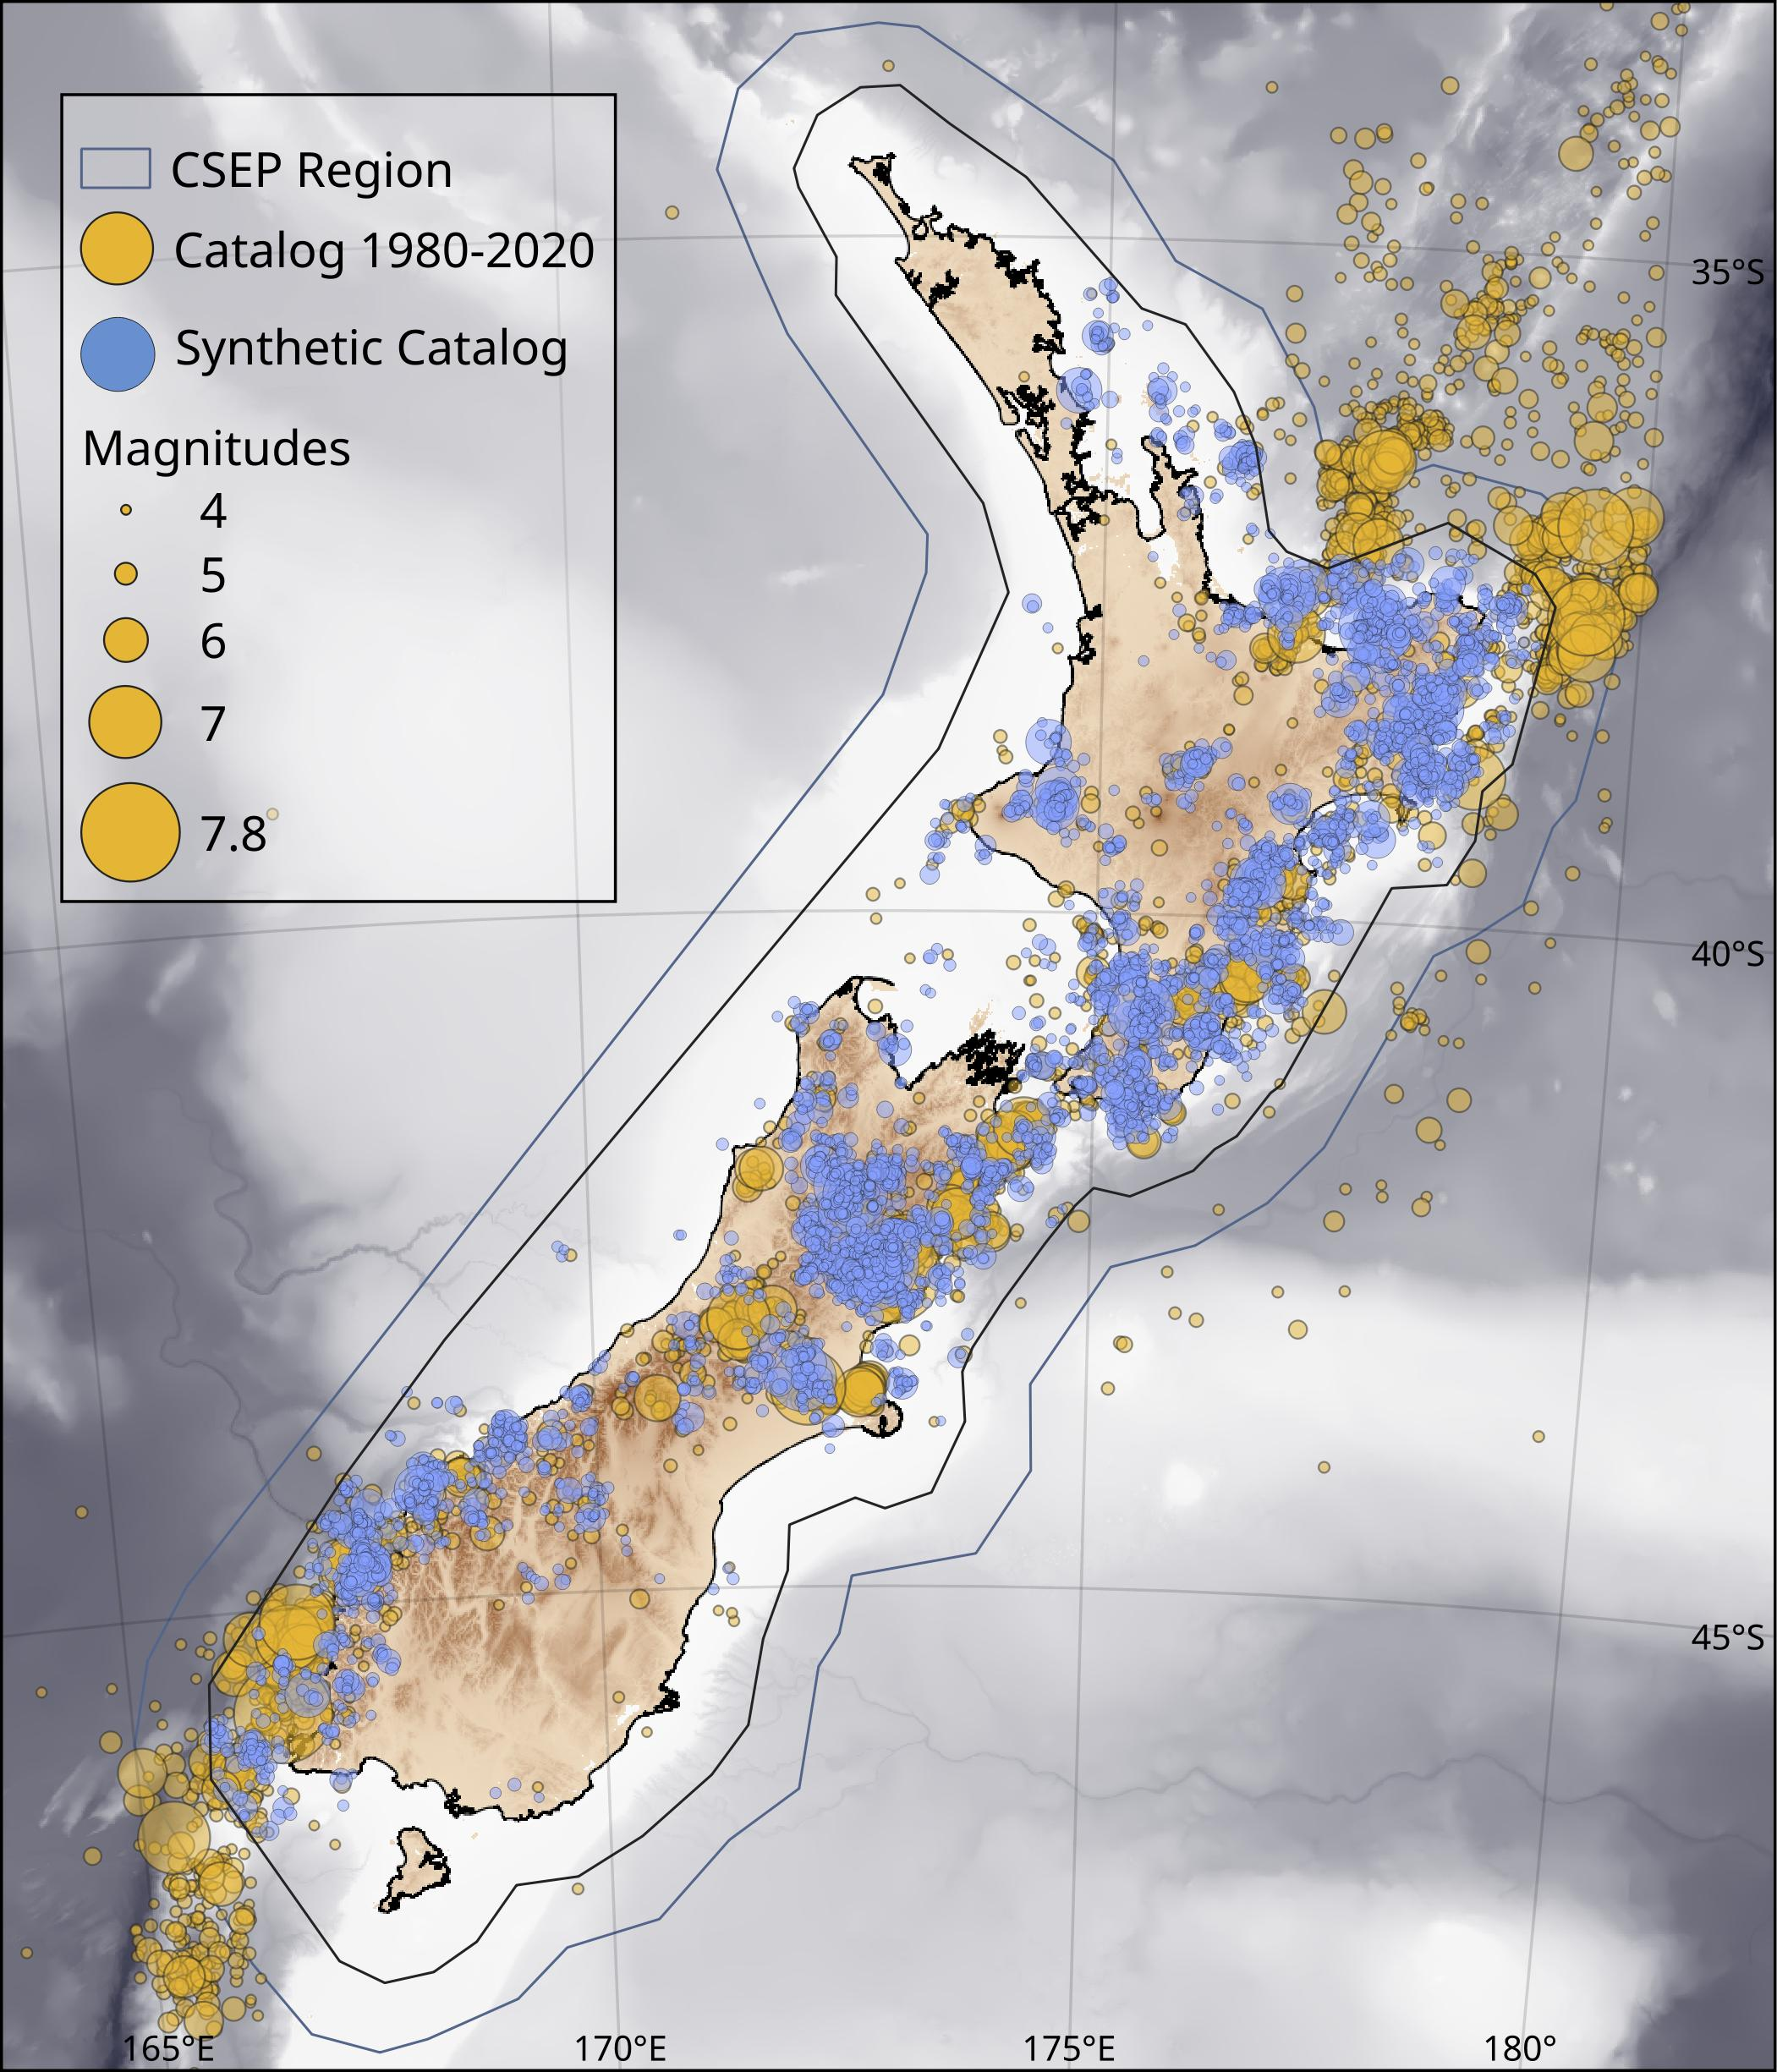
\includegraphics[width=0.9\textwidth]{./figures/catalog_forecast}
		\caption*{\scriptsize One realization of a stochastic earthquake catalog model (ETAS) for crustal seismicity in New Zealand (Iturrieta et al., 2024)}
	\end{figure}
	}
	\only<8>{
		\begin{figure}
		\vspace*{0.5cm}
		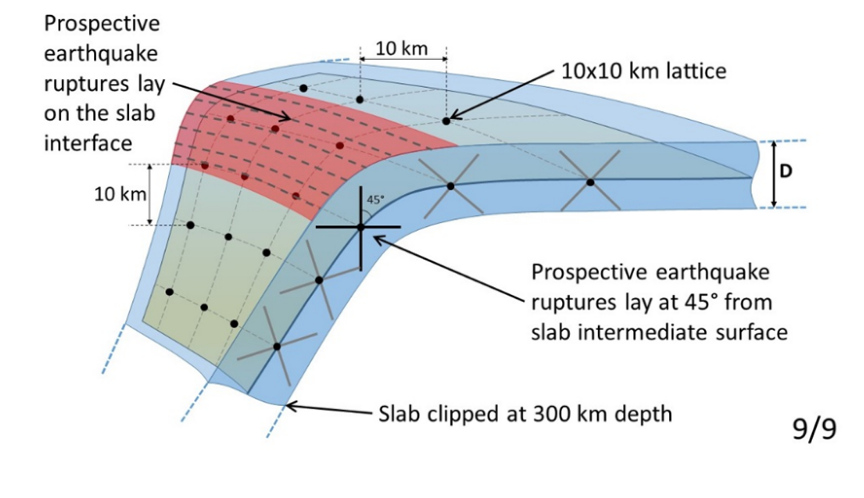
\includegraphics[width=0.95\textwidth]{./figures/subduction}
		\caption*{\scriptsize Subduction forecast, European Seismic Hazard Model ESHM2020 (Danciu et al., 2024)}
	\end{figure}
	}
	\only<9-10>{
		\begin{figure}
		\vspace*{0.5cm}
		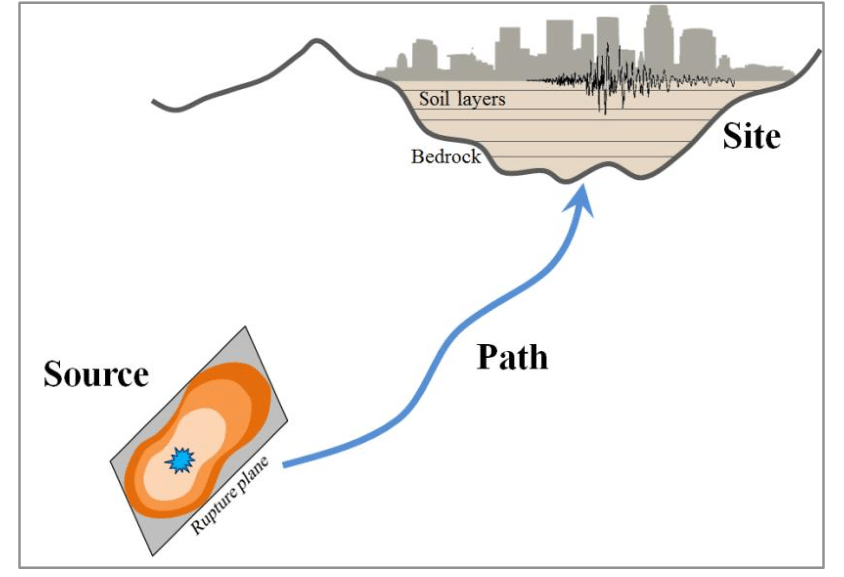
\includegraphics[width=0.95\textwidth]{./figures/gmm}
		\caption*{\scriptsize Schematic of a Ground Motion Model}
	\end{figure}
	}
	\only<11-12>{
	\begin{figure}
		\vspace*{-1.cm}
		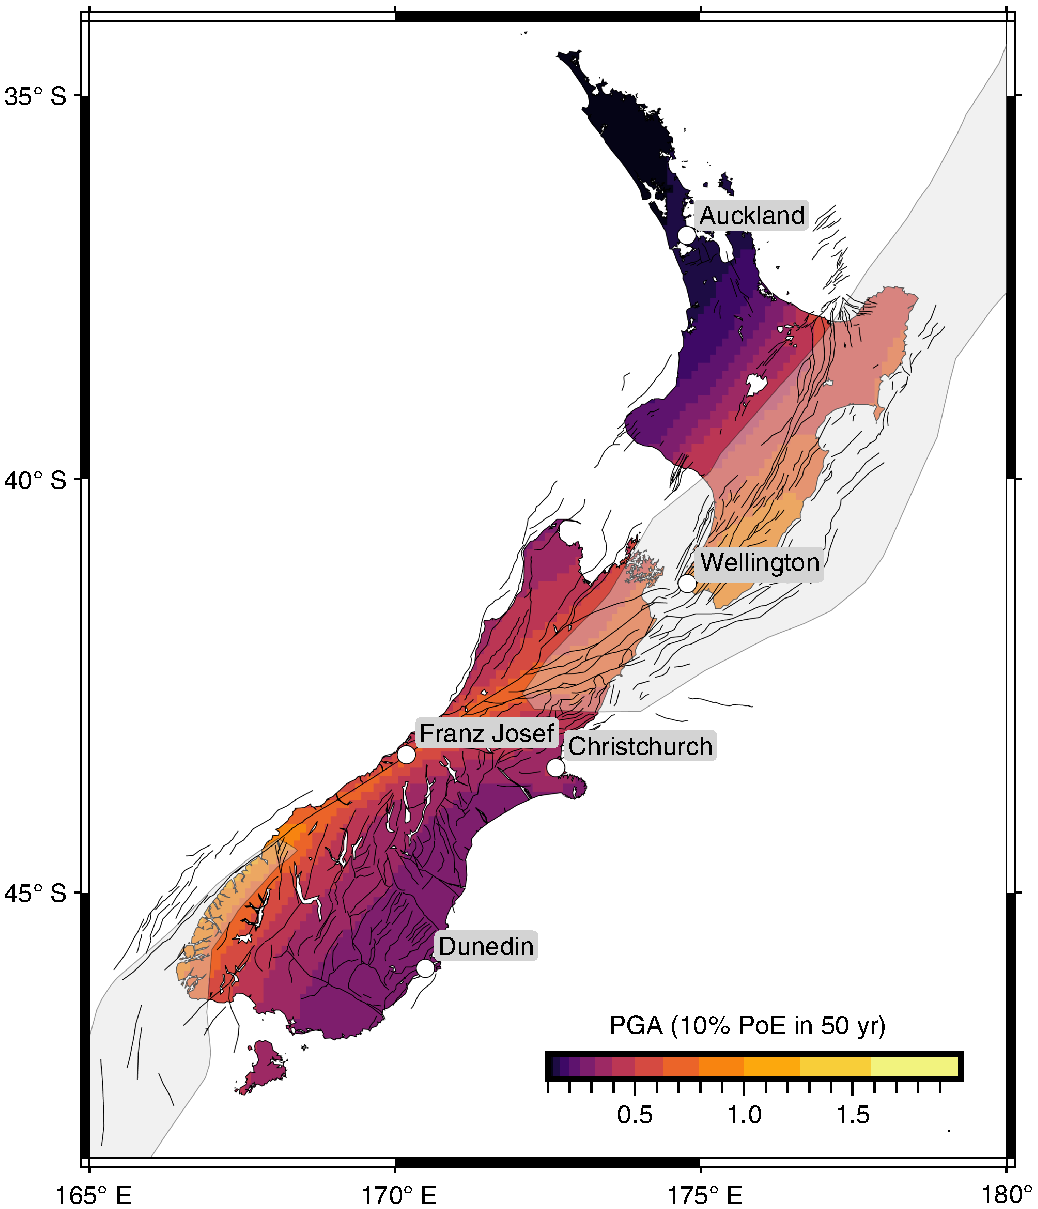
\includegraphics[width=0.85\textwidth]{./figures/hazard_model_nz}
		\caption*{\scriptsize New Zealand seismic hazard model, 2022 (Gerstenberger et al., 2023). PGA with a 10\% probability of being exceeded at least once in 50 years ($V_{\mathrm{S}30}=250 \, \mathrm{m}/\mathrm{s}$).}
	\end{figure}
	}
\end{columns}
\end{frame}

    \end{document}